\documentclass{beamer}
\usetheme{Madrid}

\usecolortheme{default}
\useinnertheme{circles}
\usepackage[brazilian]{babel}
\usepackage[utf8]{inputenc}
\usepackage{amsmath,mathtools,amsfonts,amssymb}
\usepackage{graphicx}
\usepackage{booktabs}
\usepackage{array}
\usepackage{hyperref}
\usepackage{xurl}   % quebra URLs longas (link dos pesos) sem estourar o slide

% Figuras geradas pelo pipeline
\graphicspath{{figuras/}}

% Atalho para o link de download dos pesos (Google Drive)
\newcommand{\pesoslink}{https://drive.google.com/file/d/1e6AJ6tSdS1dVmAF4KuOcWVLpn5_opASH/view?usp=drive_link}

\title[Malha Viária por Satélite]{Detecção e Reconstrução de Malha Viária a partir de Imagens de Satélite}
\subtitle{Reconhecimento de Padrões}
\author[Felipe / Igor / Victor]{Felipe Costa \and Igor Falco \and Victor Morais}
\institute[]{Reconhecimento de Padrões}
\date{\today}

\begin{document}

% ===================== CAPA =====================
\begin{frame}
    \titlepage
\end{frame}

% ===================== AGENDA =====================
\begin{frame}{Roteiro}
    \tableofcontents
\end{frame}

% =====================================================================
\section{O Problema}
% =====================================================================

\begin{frame}{Objetivo e desafios}
    \textbf{Dada uma imagem de satélite}, o sistema deve:
    \begin{enumerate}\setlength{\itemsep}{2pt}
        \item identificar as regiões que são \textbf{vias};
        \item classificar o tipo: \textbf{asfalto} ou \textbf{terra};
        \item sobrepor as vias na imagem original;
        \item extrair a \textbf{topologia} (grafo conectado: nós = cruzamentos, arestas = segmentos).
    \end{enumerate}
    \vspace{0.2cm}
    \begin{alertblock}{Por que é difícil (problema de pesquisa real)}
        \footnotesize O sistema precisa ser \textbf{robusto} a diferentes cidades, escalas, rotações, resoluções e condições visuais, \textbf{sem ajustar parâmetros para uma imagem específica}. Árvores ocultam vias; telhados, carros e solo exposto se parecem com ruas; o grafo precisa ficar \textbf{conectado}.
    \end{alertblock}
\end{frame}

\begin{frame}{Abordagem: híbrido (rede neural + visão computacional)}
    \footnotesize
    Seguimos o estado da arte (\textbf{SAM-Road}, CVPRW 2024): uma rede neural detecta as vias, e o \textbf{grafo} é a \textbf{fonte única de verdade} no pós-processamento.
    \vspace{0.15cm}
    \begin{columns}
        \column{0.5\textwidth}
        \textbf{Rede neural (aprendizado):}
        \begin{itemize}\footnotesize
            \item \textit{Vision Transformer} ViT-B (do Segment Anything, Meta).
            \item Saída: probabilidade de via + cruzamentos.
        \end{itemize}
        \column{0.5\textwidth}
        \textbf{Visão computacional (regras):}
        \begin{itemize}\footnotesize
            \item máscaras de contexto (vegetação, água, telhado, solo);
            \item grafo: pontes, podas, classificação de pavimento.
        \end{itemize}
    \end{columns}
    \vspace{0.15cm}
    \begin{block}{Contribuição própria do grupo}
        \footnotesize Pós-processamento topológico em grafo (pontes por menor custo, poda de blocos residenciais), classificação de pavimento \textbf{por aresta}, \textbf{detecção automática de domínio} (rural $\times$ urbano) e máscaras de contexto que formam os \textbf{polígonos de quarteirão}.
    \end{block}
\end{frame}

% =====================================================================
\section{Os Dados (Dataset)}
% =====================================================================

\begin{frame}[fragile]{Dataset original: SpaceNet 3 (formato SAM-Road)}
    \footnotesize
    $\sim$2.800 \textit{tiles} de 400$\times$400 px a 1\,m/pixel, em 4 cidades:
    \textbf{Las Vegas, Paris, Xangai e Cartum}. Cada \textit{tile} tem 3 arquivos:
    \vspace{0.1cm}
    \begin{tabular}{ll}
        \toprule
        \textbf{Arquivo} & \textbf{Conteúdo} \\
        \midrule
        \texttt{AOI\_2\_Vegas\_116\_\_rgb.png} & imagem de entrada (RGB) \\
        \texttt{AOI\_2\_Vegas\_116\_\_gt.png} & máscara de via (\textit{ground truth}) \\
        \texttt{AOI\_2\_Vegas\_116\_\_gt\_graph.p} & grafo de referência (\textit{pickle}) \\
        \bottomrule
    \end{tabular}
    \vspace{0.15cm}

    \begin{block}{Estrutura do grafo \texttt{.p} (dicionário de adjacência)}
        \scriptsize
\begin{verbatim}
{ (365, 152): [(352, 152), (362, 236)],   # no -> vizinhos
  (352, 152): [(365, 152), (400, 151)], ... }   # 10 nos
\end{verbatim}
    \end{block}
\end{frame}

\begin{frame}{Dataset: exemplo de um \textit{tile}}
    \begin{center}
        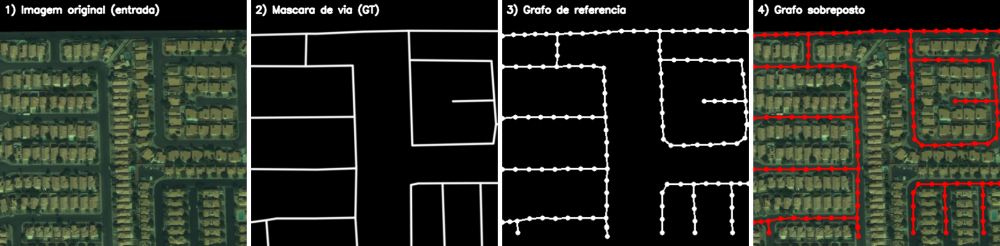
\includegraphics[width=\linewidth]{dataset_exemplo.png}
    \end{center}
    \footnotesize Da esquerda para a direita: \textbf{imagem original} (entrada), máscara de via (usada para treinar/avaliar) e o grafo de referência. As máscaras binárias \textbf{não} têm rótulo asfalto/terra --- essa classificação é feita por heurística (ver adiante).
\end{frame}

\begin{frame}{O \textit{fine-tuning} não foi realizado}
    \footnotesize
    Temos o dataset (SpaceNet 3) preparado no formato do SAM-Road e o \textit{notebook} de treino pronto, \textbf{mas o ajuste fino (\textit{fine-tuning}) não foi executado}:
    \begin{itemize}\setlength{\itemsep}{3pt}
        \item \textbf{Sem GPU local} para treinar uma ViT-B ($\sim$90\,M de parâmetros);
        \item o \textbf{Google Colab} gratuito \textbf{limita a sessão a $\sim$4\,h}, insuficiente para uma época completa estável neste modelo.
    \end{itemize}
    \vspace{0.1cm}
    \begin{block}{Consequência}
        \scriptsize Usamos os \textbf{pesos pré-treinados} (CityScale). Tudo o que apresentamos é a \textbf{engenharia de inferência e o pós-processamento} sobre esses pesos --- onde está a contribuição do grupo. O \textit{fine-tuning} fica como trabalho futuro (notebook em \texttt{training/}).
    \end{block}
\end{frame}

% =====================================================================
\section{O Modelo e os Pesos}
% =====================================================================

\begin{frame}[fragile]{Documentação dos pesos pré-treinados}
    \footnotesize
    O \textit{checkpoint} \texttt{cityscale\_vitb\_512\_e10.ckpt} ($\sim$1\,GB) é o SAM-Road ajustado. O dicionário de pesos tem \textbf{229 tensores} em 3 ramos:
    \vspace{0.1cm}
    \begin{tabular}{lrl}
        \toprule
        \textbf{Ramo (prefixo)} & \textbf{Tensores} & \textbf{Papel} \\
        \midrule
        \texttt{image\_encoder.*} & 177 & encoder ViT-B (features) \\
        \texttt{map\_decoder.*} & 10 & via + cruzamentos (\textbf{usado}) \\
        \texttt{topo\_net.*} & 42 & topologia (não usado) \\
        \bottomrule
    \end{tabular}
    \vspace{0.1cm}
    \begin{block}{Download dos pesos (não vão no repositório)}
        \scriptsize Baixe \texttt{cityscale\_vitb\_512\_e10.ckpt} e coloque em \texttt{weights/}:\\
        \href{\pesoslink}{\textbf{Google Drive --- baixar pesos}} \\[2pt]
        {\tiny\url{\pesoslink}}
    \end{block}
\end{frame}

\begin{frame}[fragile]{Limiares do pipeline (fixos / adaptativos por domínio)}
    \footnotesize Os limiares de \textbf{detecção} são absolutos (iguais para qualquer imagem); o limiar de \textbf{pavimento} é \textbf{adaptado automaticamente} ao domínio detectado --- nunca ajustado à mão por imagem.
    \vspace{0.1cm}
    \begin{tabular}{lll}
        \toprule
        \textbf{Limiar} & \textbf{Valor} & \textbf{Onde / para quê} \\
        \midrule
        \texttt{ROAD\_THRESHOLD} & 0,341 & operating point do modelo \\
        \texttt{HYST\_HIGH} & 0,30 & semente forte (hysteresis) \\
        \texttt{HYST\_LOW} & 0,04 & trecho fraco conectado \\
        \texttt{TERRA\_THR (urbano)} & 0,45 & asfalto $\times$ terra (denso) \\
        \texttt{TERRA\_THR (rural)} & 0,20 & asfalto $\times$ terra (rural) \\
        \bottomrule
    \end{tabular}
    \vspace{0.1cm}
    \begin{block}{Regime de sinal fraco (robustez de domínio)}
        \scriptsize Se a probabilidade máxima fica entre 0,10 e 0,30 (ex.: satélite escuro fora do treino), os limiares viram \textbf{relativos} ($0{,}45\times$ e $0{,}12\times$ o máximo). Abaixo de 0,10, retorna ``sem vias'' (não amplifica ruído).
    \end{block}
\end{frame}

% =====================================================================
\section{Pipeline Passo a Passo}
% =====================================================================

\begin{frame}{Visão geral do pipeline (9 passos)}
    \footnotesize
    \begin{enumerate}\setlength{\itemsep}{1pt}
        \item \textbf{Original} --- imagem de entrada.
        \item \textbf{Pré-processamento} (realce de bordas \textit{canny}) --- só para a rede.
        \item \textbf{Probabilidade do modelo} --- inferência multi-escala (\textit{upscale} 2$\times$ p/ vias finas).
        \item \textbf{Máscaras de contexto} --- vegetação, água, \textbf{quarteirões}, solo.
        \item \textbf{Probabilidade suprimida} --- contexto rebaixa regiões improváveis.
        \item \textbf{Binarização} (hysteresis) $\rightarrow$ esqueleto.
        \item \textbf{Grafo bruto} do esqueleto.
        \item \textbf{Grafo refinado} --- pontes, poda de pontas e blocos.
        \item \textbf{Overlay final} --- classificação por aresta (asfalto/terra).
    \end{enumerate}
    \vspace{0.05cm}
    \begin{alertblock}{Detalhe importante}
        \scriptsize O realce \textit{canny} alimenta \textbf{apenas a rede}. Classificação de pavimento, máscaras e desenho usam sempre a imagem \textbf{original} --- bordas sintéticas não podem virar ``terra''.
    \end{alertblock}
\end{frame}

\begin{frame}{Passo 1--3: original, pré-processamento e inferência}
    \begin{columns}
        \column{0.5\textwidth}
        \begin{center}
            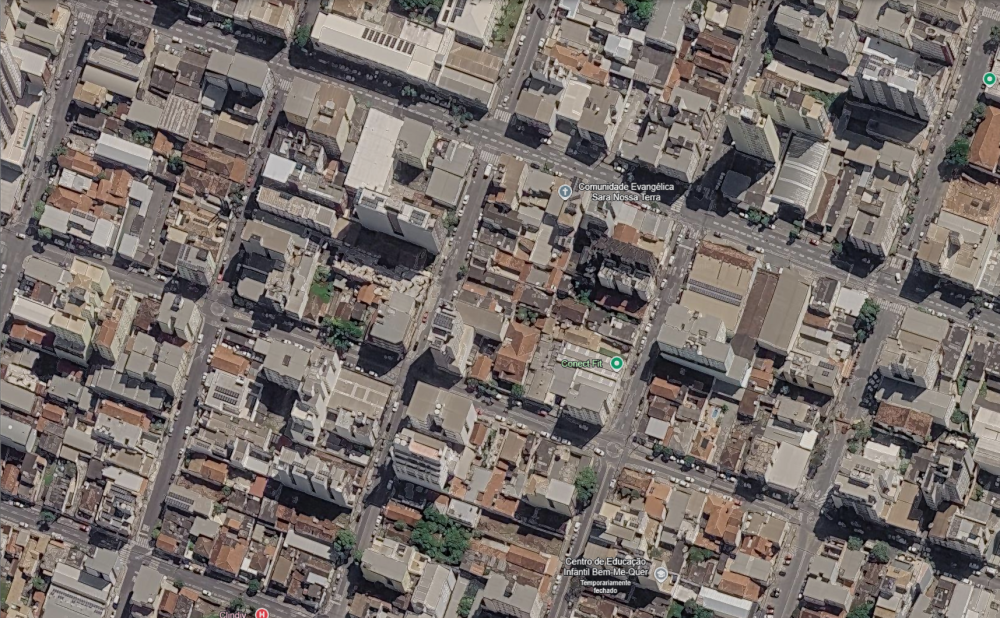
\includegraphics[width=\linewidth]{2_preprocessamento_canny.png}\\[2pt]
            \scriptsize \textbf{Realce \textit{canny}} (entrada da rede).
        \end{center}
        \column{0.5\textwidth}
        \begin{center}
            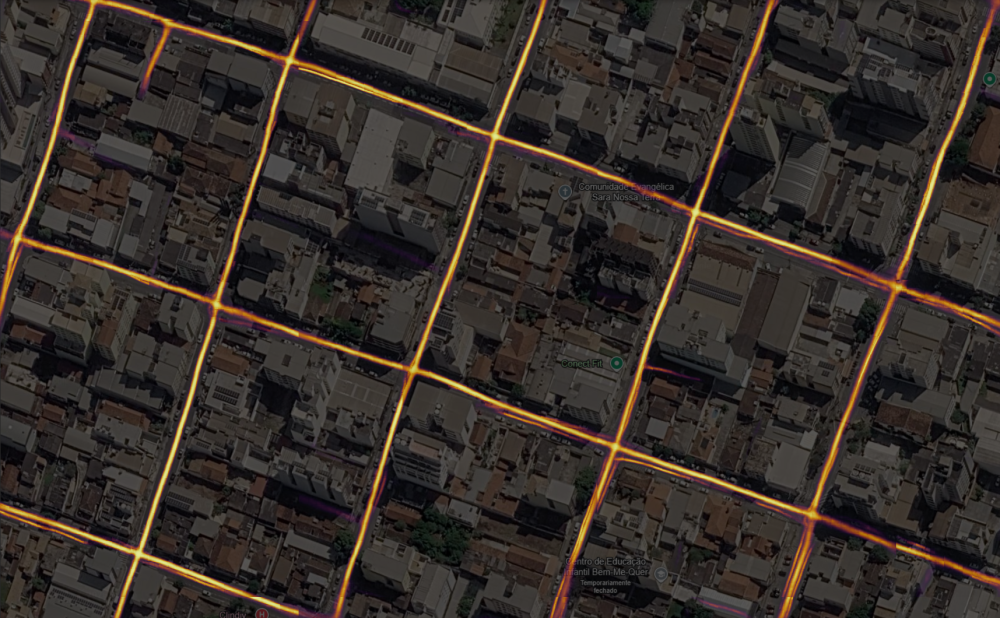
\includegraphics[width=\linewidth]{3_probabilidade_modelo.png}\\[2pt]
            \scriptsize \textbf{Probabilidade de via} (mapa de calor da rede).
        \end{center}
    \end{columns}
    \vspace{0.1cm}
    \footnotesize A rede (ViT-B) processa a imagem em janelas de 512$\times$512 com 50\% de sobreposição, em 2 escalas. A fusão por máximo preserva vias finas e largas.
\end{frame}

\begin{frame}{Passo 4: máscaras de contexto (legenda de cores)}
    \begin{columns}
        \column{0.54\textwidth}
        \begin{center}
            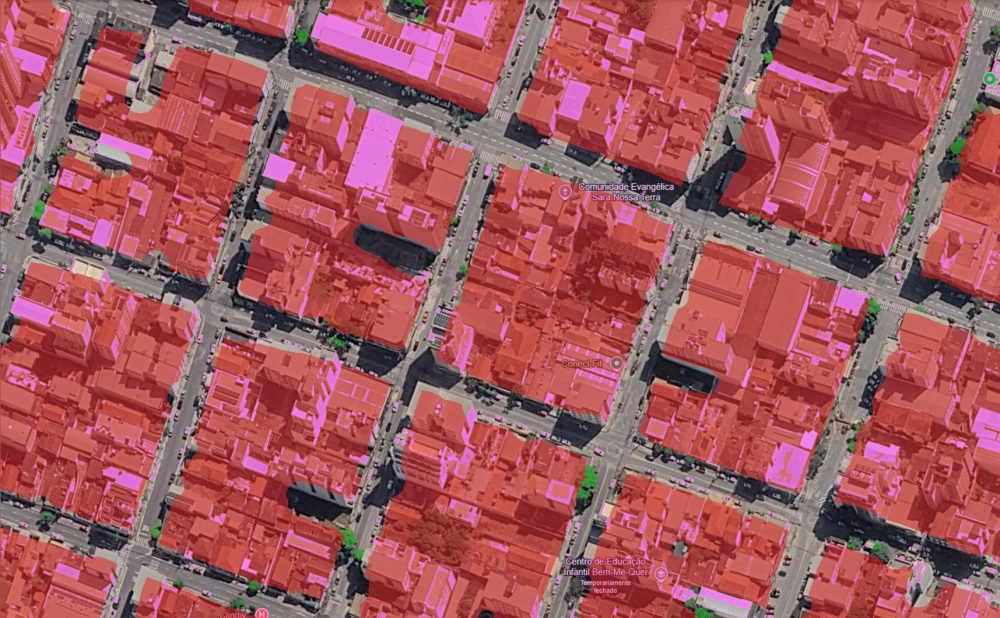
\includegraphics[width=\linewidth]{4_mascaras_contexto.png}
        \end{center}
        \column{0.46\textwidth}
        \scriptsize
        \textbf{Cada cor = um detector de contexto:}
        \vspace{0.1cm}
        \begin{tabular}{ll}
            \toprule
            \textbf{Cor} & \textbf{Detecta} \\
            \midrule
            \textcolor{green!60!black}{$\blacksquare$ Verde} & vegetação \\
            \textcolor{blue}{$\blacksquare$ Azul} & água \\
            \textcolor{red}{$\blacksquare$ Vermelho} & telhado / quarteirão \\
            \textcolor{yellow!85!black}{$\blacksquare$ Amarelo} & solo exposto \\
            \textcolor{magenta}{$\blacksquare$ Rosa} & rejeição por brilho \\
            \bottomrule
        \end{tabular}
        \vspace{0.1cm}

        O quarteirão é marcado \textbf{inteiro}, mas as \textbf{vias são recortadas} pela probabilidade do modelo --- carro/rua sobre o bloco não viram telhado.
    \end{columns}
\end{frame}

\begin{frame}{Detecção automática de domínio: rural $\times$ urbano}
    \footnotesize
    O mesmo pipeline atende cenas opostas. Em vez de um botão manual, o sistema \textbf{decide sozinho} pela imagem:
    \vspace{0.1cm}
    \[
        \text{rural} \;\Longleftrightarrow\; \underbrace{\text{vegetação} > 25\%}_{\text{muito verde}} \;\;\textbf{E}\;\; \underbrace{\text{densidade de via} < 1{,}2\%}_{\text{malha esparsa}}
    \]
    \begin{block}{Por que as duas condições juntas}
        \scriptsize Vegetação sozinha engana: uma \textbf{favela em vale verde} tem $\sim$40\% de verde \textbf{mas} malha densa ($\sim$3,5\%) --- é \textbf{urbana}. A densidade separa limpo: rural $\le$0,6\% vs.\ favela/urbano $\ge$2\%.
    \end{block}
    \vspace{0.05cm}
    \begin{columns}
        \column{0.5\textwidth}
        \scriptsize\textbf{Rural} $\Rightarrow$ pula refino; telhado/solo \textbf{off}; \texttt{TERRA\_THR}=0,20 (pega terra fina).
        \column{0.5\textwidth}
        \scriptsize\textbf{Urbano} $\Rightarrow$ refino \textbf{on}; telhado \textbf{on}; \texttt{TERRA\_THR}=0,45 (evita asfalto-fino virar laranja).
    \end{columns}
\end{frame}

\begin{frame}{Passo 5--7: supressão, binarização e grafo bruto}
    \begin{columns}
        \column{0.5\textwidth}
        \begin{center}
            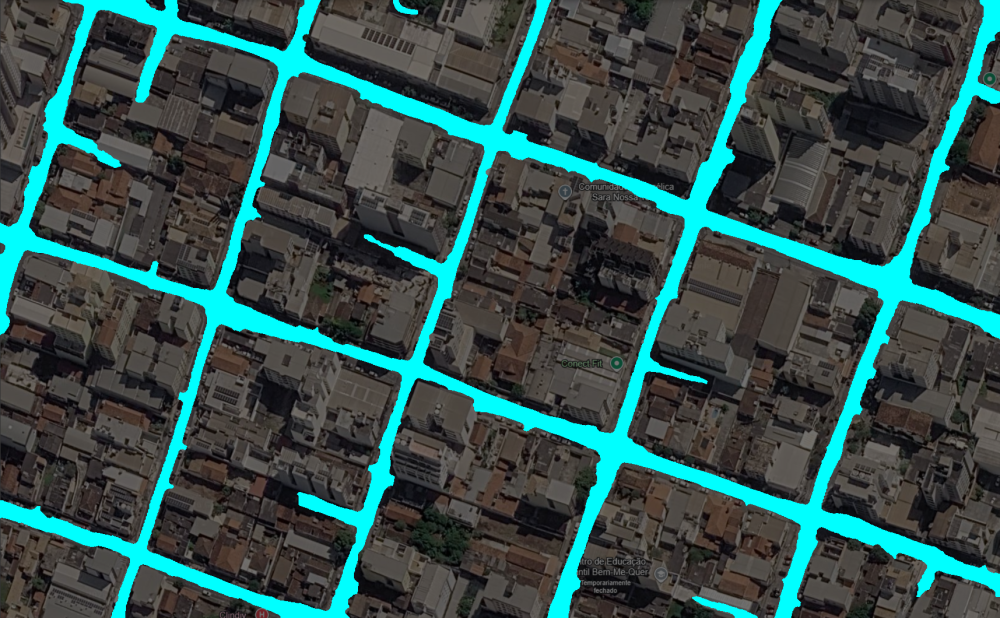
\includegraphics[width=\linewidth]{6_binaria.png}\\[2pt]
            \scriptsize \textbf{Máscara binária} (hysteresis).
        \end{center}
        \column{0.5\textwidth}
        \begin{center}
            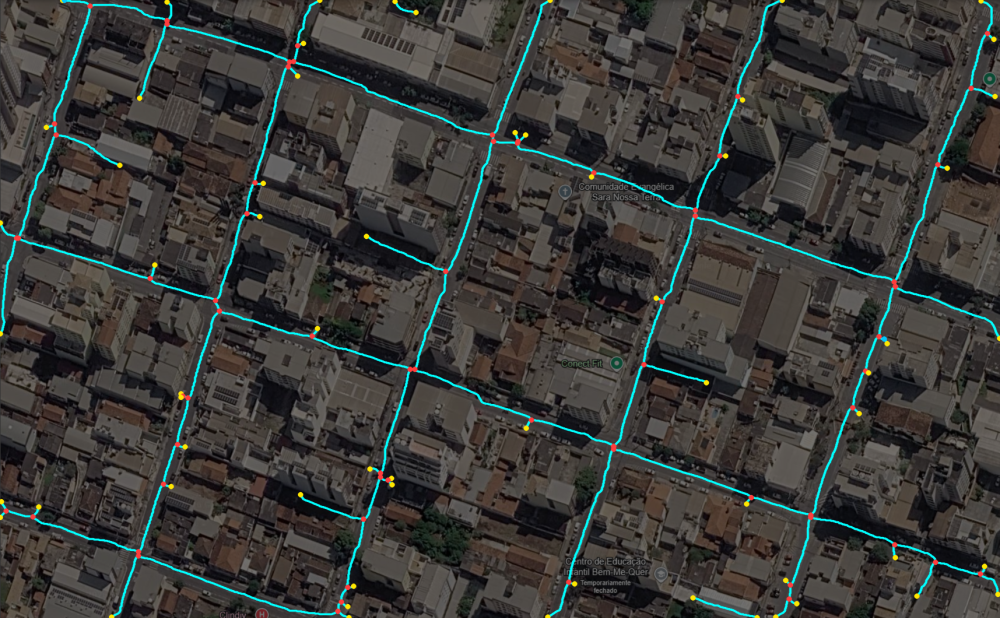
\includegraphics[width=\linewidth]{7_grafo_bruto.png}\\[2pt]
            \scriptsize \textbf{Grafo bruto} do esqueleto.
        \end{center}
    \end{columns}
    \vspace{0.1cm}
    \footnotesize A probabilidade suprimida pelo contexto é binarizada por \textbf{hysteresis} e esqueletizada $\rightarrow$ grafo: \textcolor{red}{nós vermelhos} = cruzamentos, \textcolor{yellow!80!black}{amarelos} = pontas. Ainda há pontas soltas e fragmentos a corrigir.
\end{frame}

\begin{frame}{Passo 8: refino do grafo}
    \begin{columns}
        \column{0.56\textwidth}
        \begin{center}
            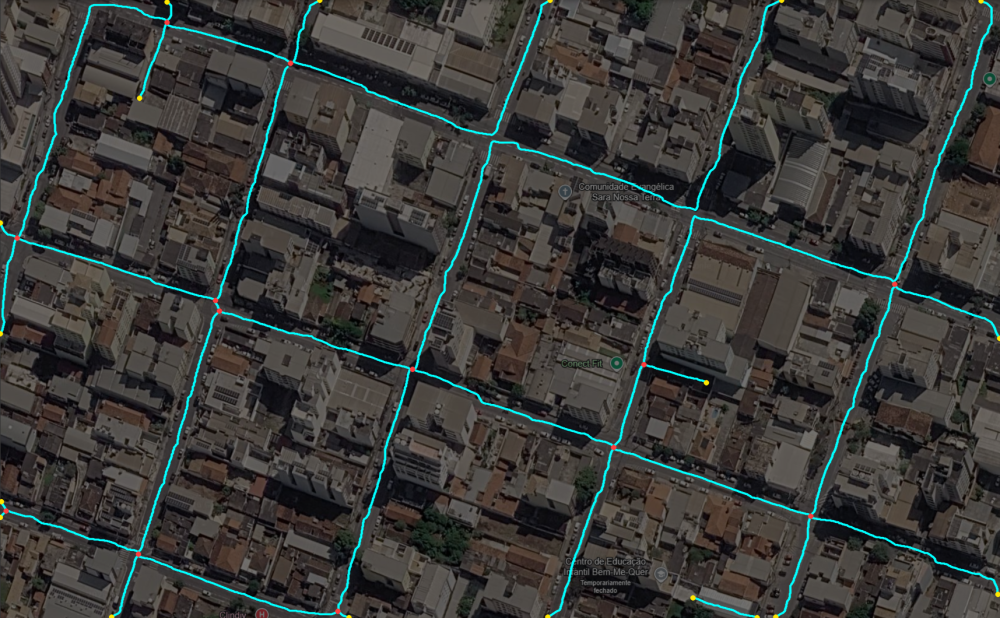
\includegraphics[width=\linewidth]{8_grafo_refinado.png}
        \end{center}
        \column{0.44\textwidth}
        \footnotesize
        \textbf{Correções (todas no grafo):}
        \begin{itemize}\scriptsize
            \item \textbf{pontes}: conecta buracos por caminho de menor custo (Dijkstra) sobre $1/\text{prob}$;
            \item \textbf{poda de pontas} curtas e de pontas em telhado (``via dentro de casa'');
            \item \textbf{toco de quarteirão}: remove aresta de ponta solta presa dentro de um bloco;
            \item \textbf{loops falsos}: apaga conector curto redundante;
            \item \textbf{terra isolada}: aresta de terra cercada só por asfalto vira asfalto.
        \end{itemize}
        \scriptsize\textit{Em cenas muito verdes o refino é pulado} (calibrado p/ urbano).
    \end{columns}
\end{frame}

\begin{frame}{Passo 9: classificação por aresta e overlay}
    \begin{columns}
        \column{0.56\textwidth}
        \begin{center}
            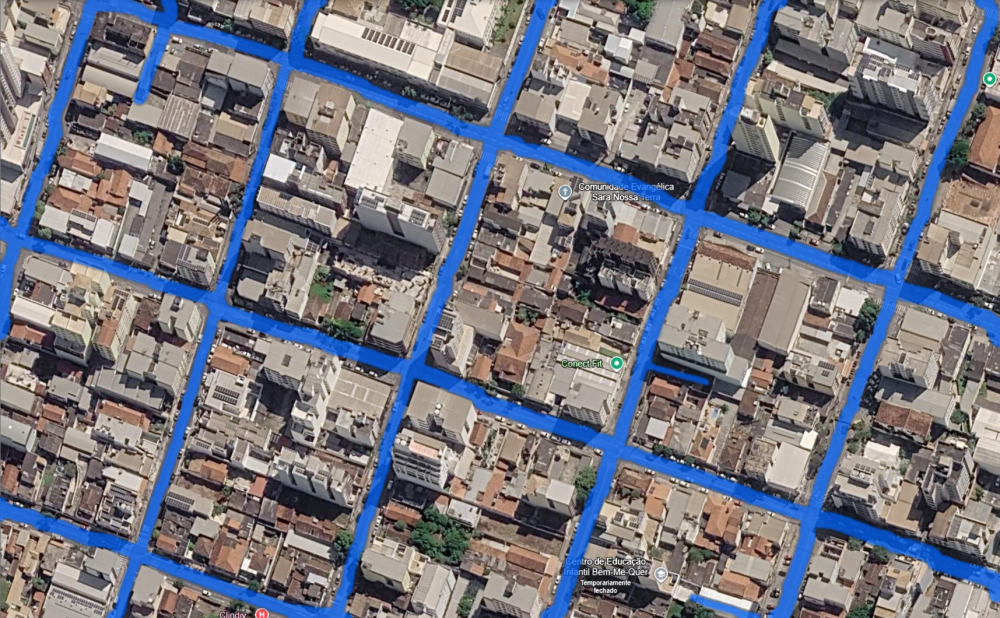
\includegraphics[width=\linewidth]{9_overlay_final.png}
        \end{center}
        \column{0.44\textwidth}
        \footnotesize
        A classe (\textbf{\textcolor{blue}{asfalto}} / \textbf{\textcolor{orange}{terra}}) é decidida \textbf{por aresta inteira} (percentil da evidência cor+textura no núcleo da via), não pixel a pixel --- evita o efeito ``zebra''.
        \vspace{0.1cm}

        O limiar terra/asfalto é o \textbf{adaptativo por domínio}. Uma suavização (ICM) faz vias contínuas terem a mesma classe; trocas \textbf{reais} de pavimento viram um nó de transição.
        \begin{block}{Saídas}
            \scriptsize overlay, máscara, e o \textbf{grafo} em JSON + GraphML (nós, arestas, pavimento, largura, comprimento).
        \end{block}
    \end{columns}
\end{frame}

% =====================================================================
\section{Resultados}
% =====================================================================

\begin{frame}{Avaliação quantitativa (com \textit{ground truth})}
    \footnotesize
    Avaliação com \textit{ground truth} (12 \textit{tiles} do SpaceNet, buffer de 8\,px), comparando o pós-processamento em grafo com o método anterior (\textbf{mesmo modelo}):
    \vspace{0.15cm}
    \begin{tabular}{lccccc}
        \toprule
        \textbf{Método} & \textbf{Precisão} & \textbf{Recall} & \textbf{F1} & \textbf{FP (px)} & \textbf{Pontas} \\
        \midrule
        Anterior (pixel) & 0,671 & 0,894 & 0,751 & 4228 & 15,2 \\
        \textbf{Grafo (nosso)} & \textbf{0,890} & \textbf{0,942} & \textbf{0,909} & \textbf{1960} & \textbf{11,3} \\
        \bottomrule
    \end{tabular}
    \vspace{0.2cm}
    \begin{itemize}\footnotesize
        \item \textbf{+15,8 pontos de F1}, falsos positivos pela metade, menos pontas soltas.
        \item A poda urbana custou apenas $-0{,}9$ de F1 e cortou $14\%$ dos falsos positivos.
        \item A seguir: \textbf{avaliação qualitativa} --- os 9 passos de cada imagem de teste.
    \end{itemize}
\end{frame}

% --------- GRADES DE PASSOS POR IMAGEM (4 em cima, 5 embaixo) ---------

\begin{frame}{Resultado --- 135241 (urbano denso)}
    \begin{center}
        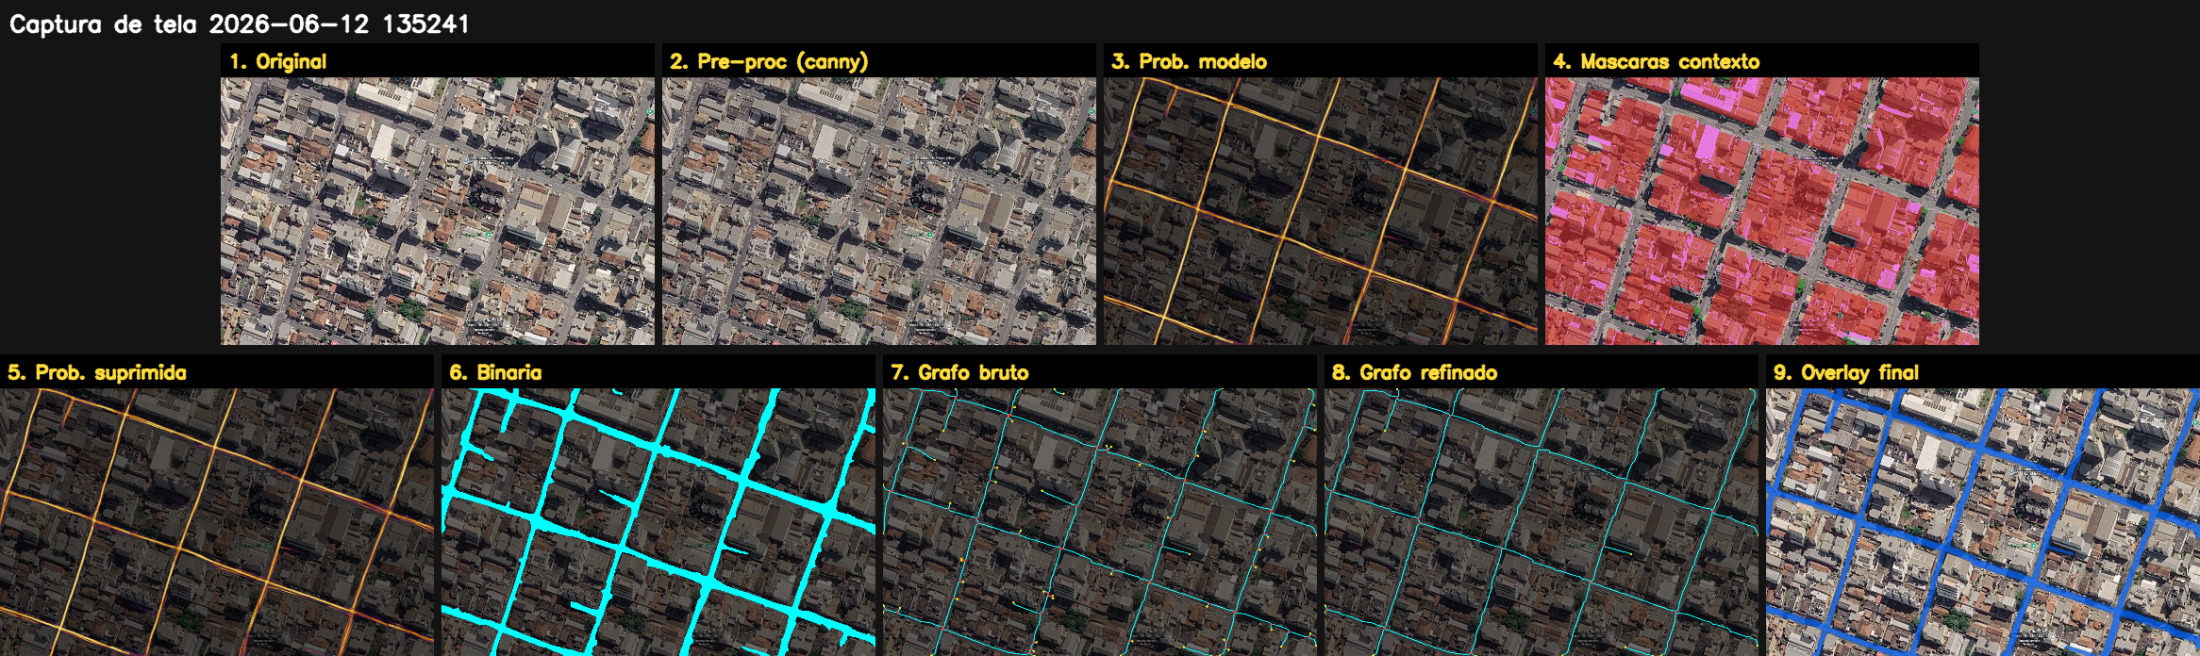
\includegraphics[width=\linewidth]{grid_2026-06-12_135241.png}
    \end{center}
    \footnotesize Ambiente urbano \textbf{densamente residencial}. A malha de asfalto foi extraída de forma \textbf{perfeita}: totalmente conectada, em azul, sem tocos nem falsos positivos. (Avaliação do grupo: ``muito bom''.)
\end{frame}

\begin{frame}{Resultado --- 020059 (avenidas asfaltadas)}
    \begin{center}
        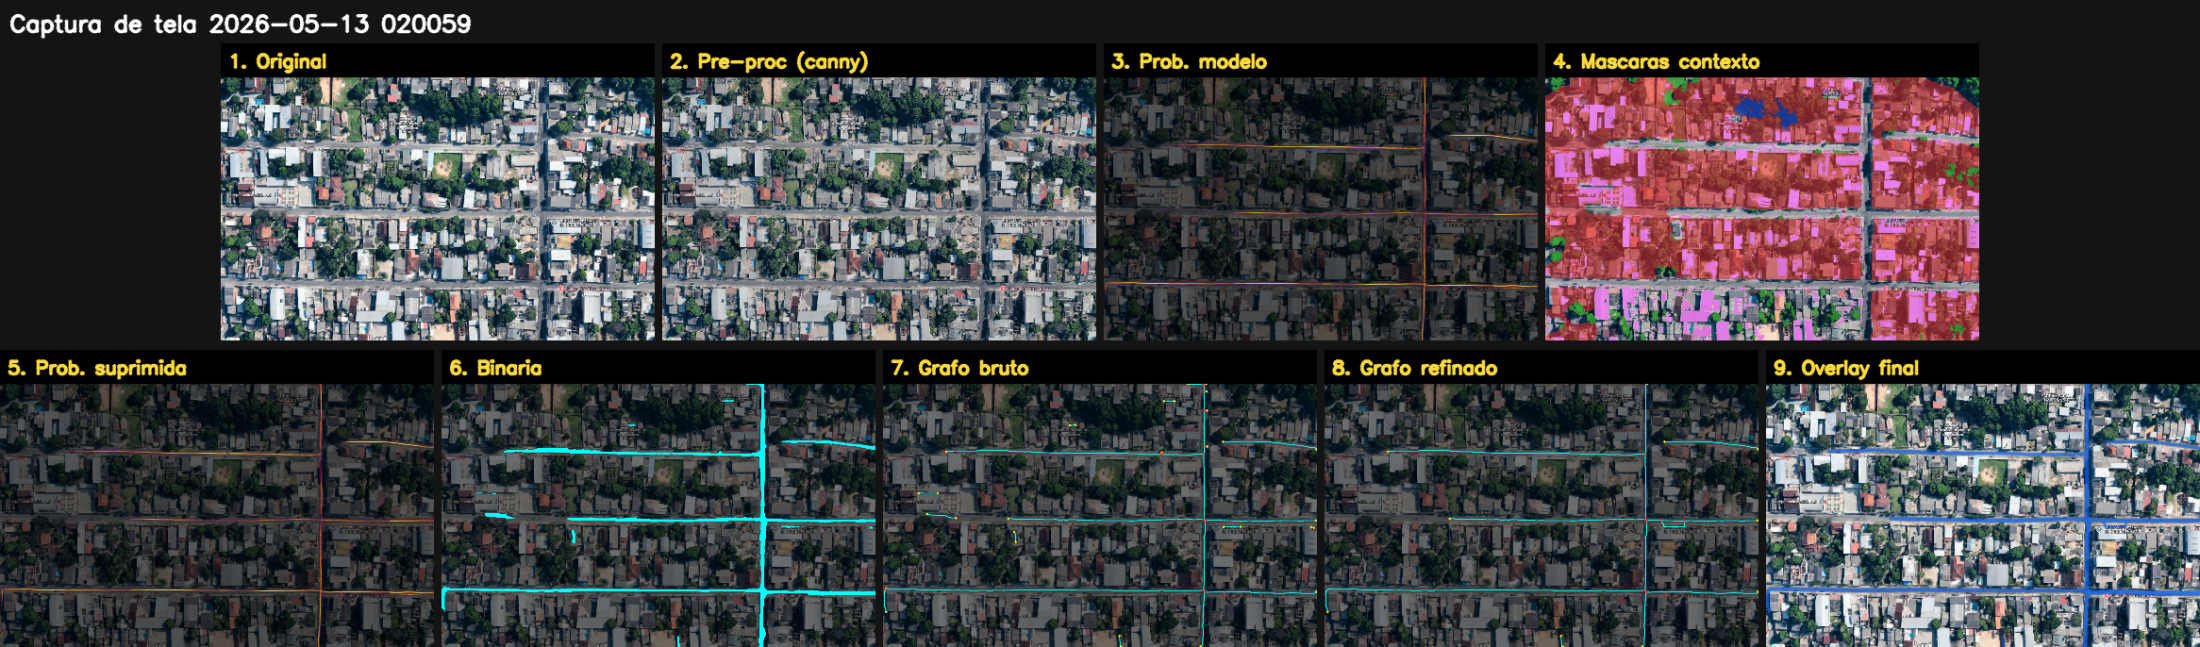
\includegraphics[width=\linewidth]{grid_2026-05-13_020059.png}
    \end{center}
    \footnotesize Tecido urbano denso com avenidas em azul (asfalto). Após a correção, o \textbf{telhado não invade mais as vias}: a supressão de telhado virou \textbf{suave} e as vias detectadas são recortadas da máscara de quarteirão.
\end{frame}

\begin{frame}{Resultado --- 151237 (favela em vale verde)}
    \begin{center}
        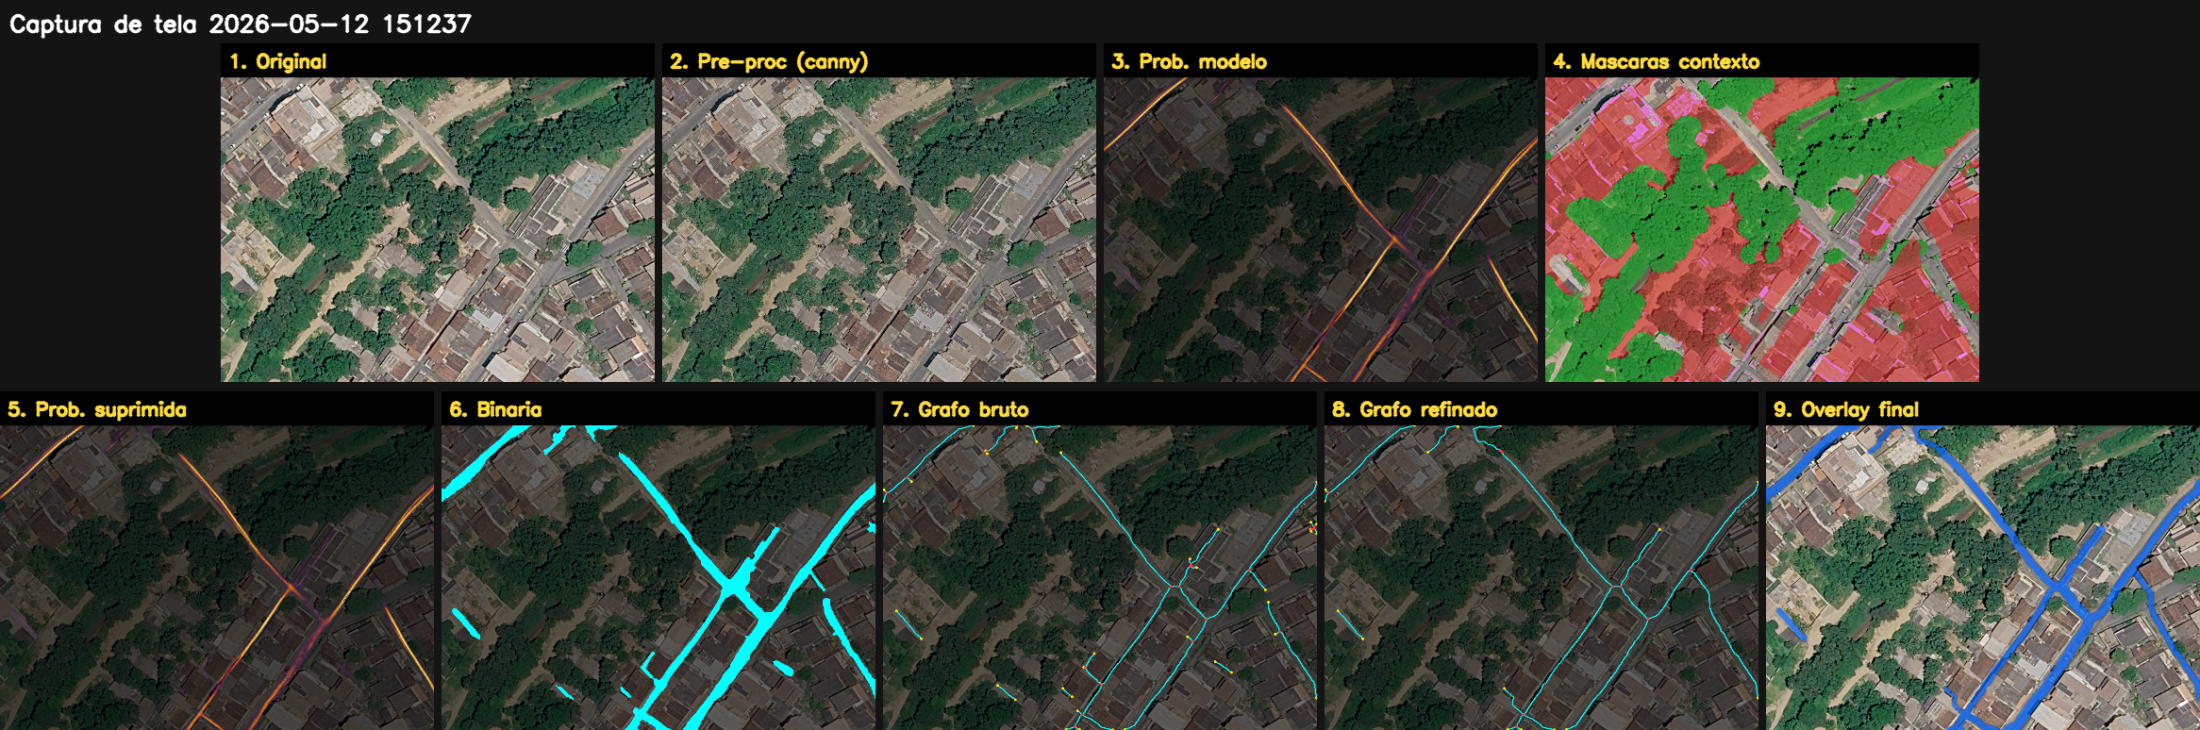
\includegraphics[width=\linewidth]{grid_2026-05-12_151237.png}
    \end{center}
    \footnotesize Mesmo com $\sim$40\% de vegetação, a \textbf{densidade da malha} indica domínio \textbf{urbano}: o asfalto é classificado corretamente em \textbf{azul} (antes saía laranja) e \textbf{não há tocos de terra soltos} no meio do asfalto.
\end{frame}

\begin{frame}{Resultado --- 003536 (núcleos densos na mata)}
    \begin{center}
        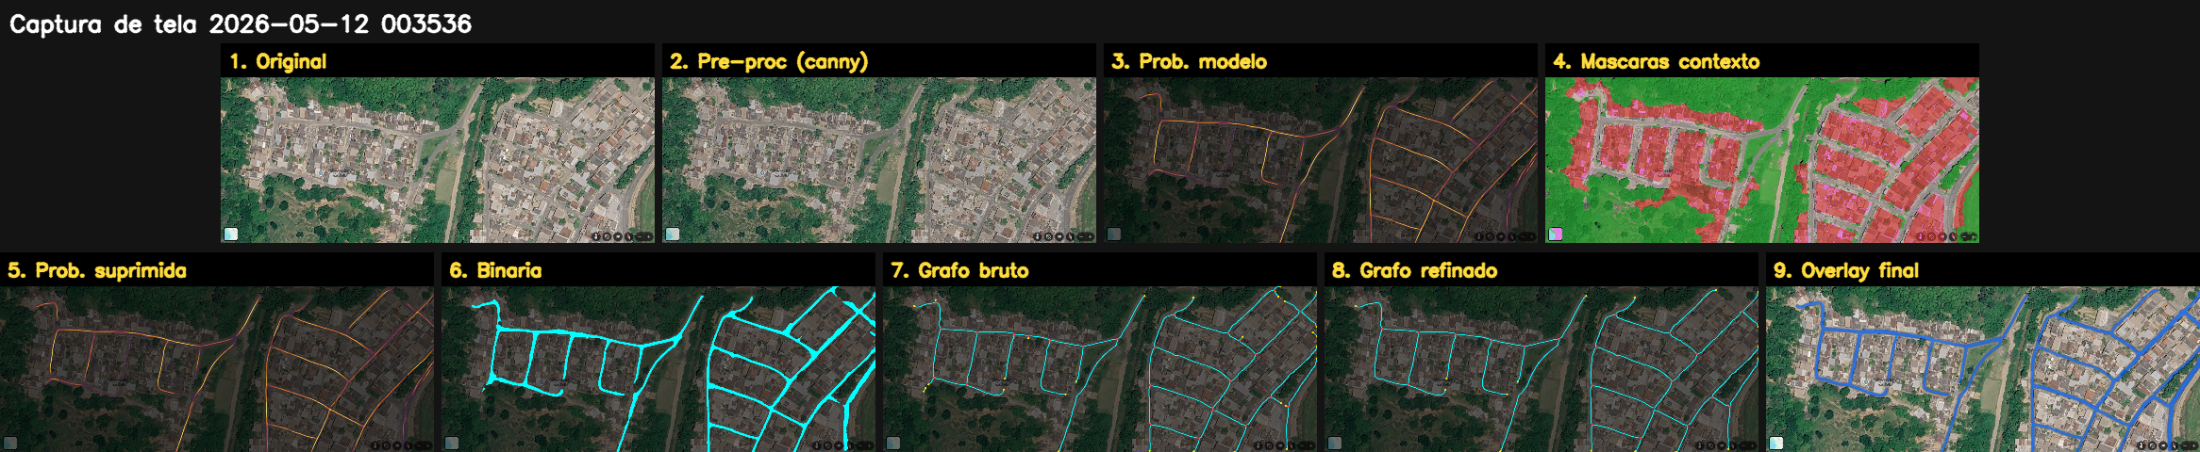
\includegraphics[width=\linewidth]{grid_2026-05-12_003536.png}
    \end{center}
    \footnotesize Dois núcleos urbanos densos cercados por vegetação. A detecção de domínio por densidade os trata como \textbf{urbanos}; a malha sai conectada em azul, sem confundir mata com via.
\end{frame}

\begin{frame}{Resultado --- 202053 (rural: terra + asfalto + água)}
    \begin{center}
        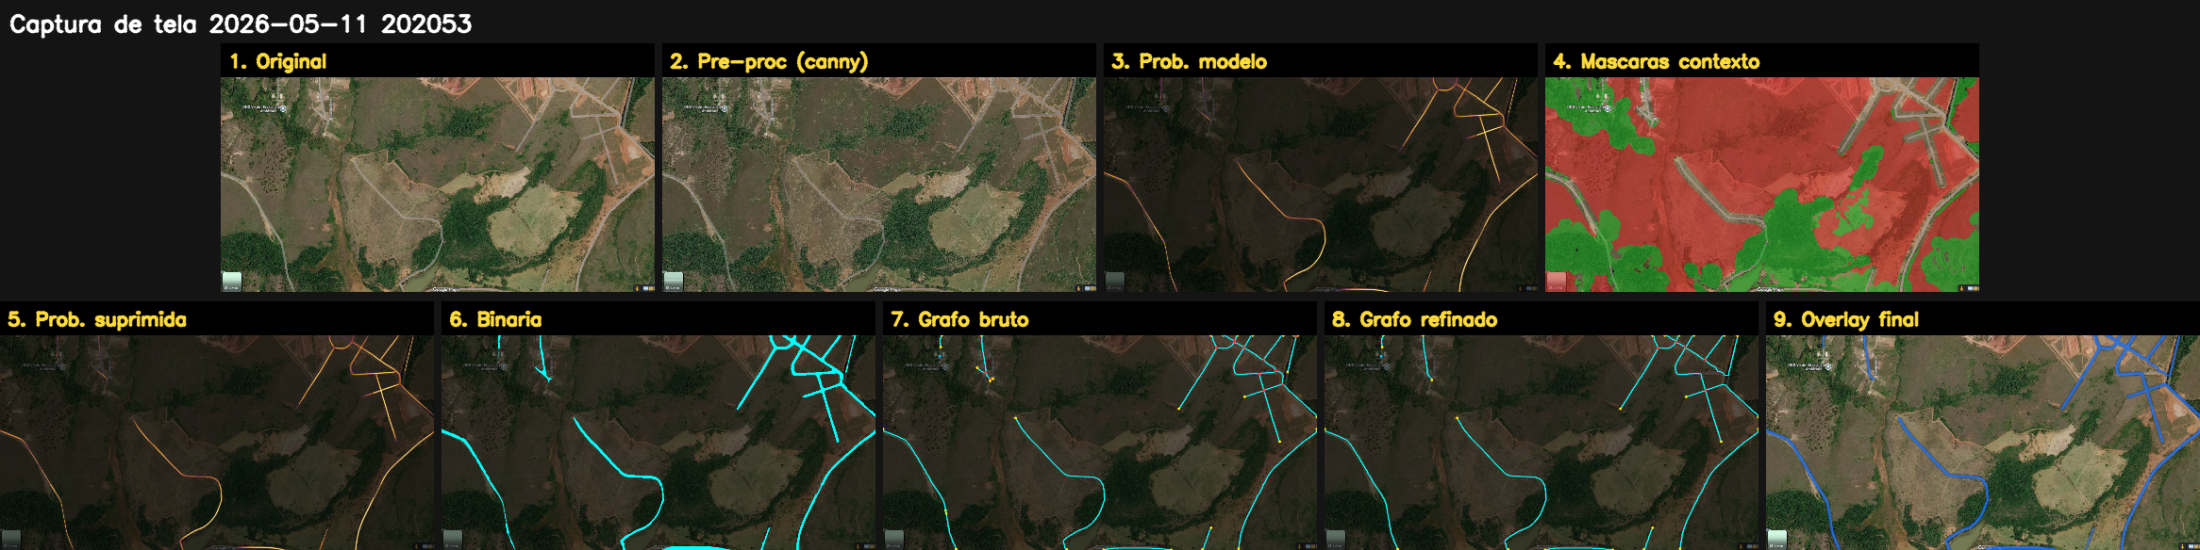
\includegraphics[width=\linewidth]{grid_2026-05-11_202053.png}
    \end{center}
    \footnotesize Cena rural com vegetação densa: vias de \textbf{terra} (laranja) e \textbf{asfalto} (azul) coexistem, e a \textbf{água} é detectada (canto superior). Por ser muito verde, o \textbf{refino é pulado} para não comer as vias de terra finas.
\end{frame}

\begin{frame}{Resultado --- 131959 (rural)}
    \begin{center}
        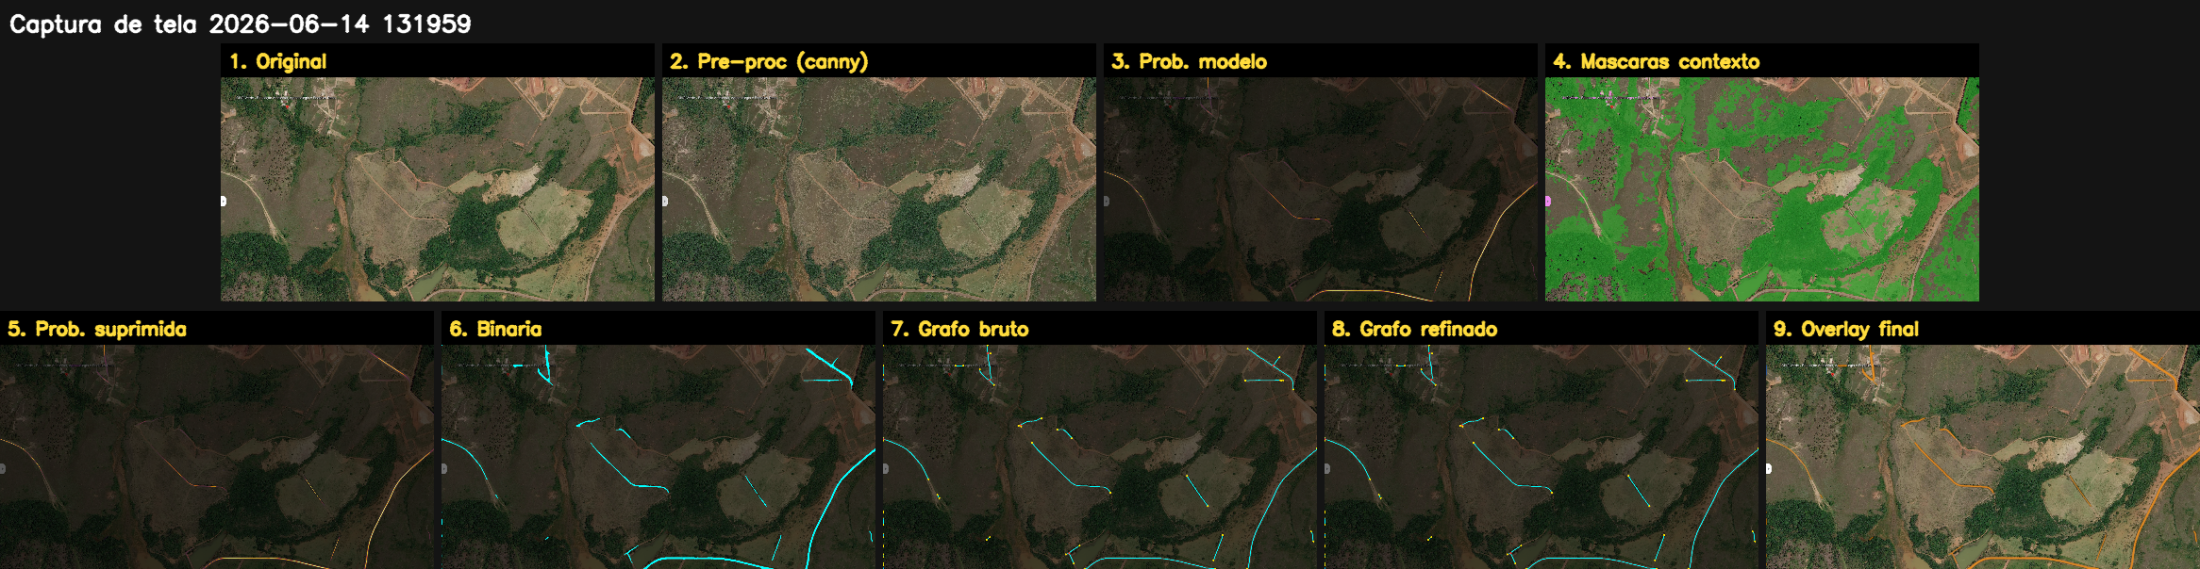
\includegraphics[width=\linewidth]{grid_2026-06-14_131959.png}
    \end{center}
    \footnotesize Domínio \textbf{rural} (alta vegetação + malha esparsa). As vias de terra foram bem classificadas em \textbf{laranja}; \textbf{funcionou bem, mas algumas vias ficaram incompletas} por terem textura/contraste fraco.
\end{frame}

\begin{frame}{Resultado --- 165358 (rural misto)}
    \begin{center}
        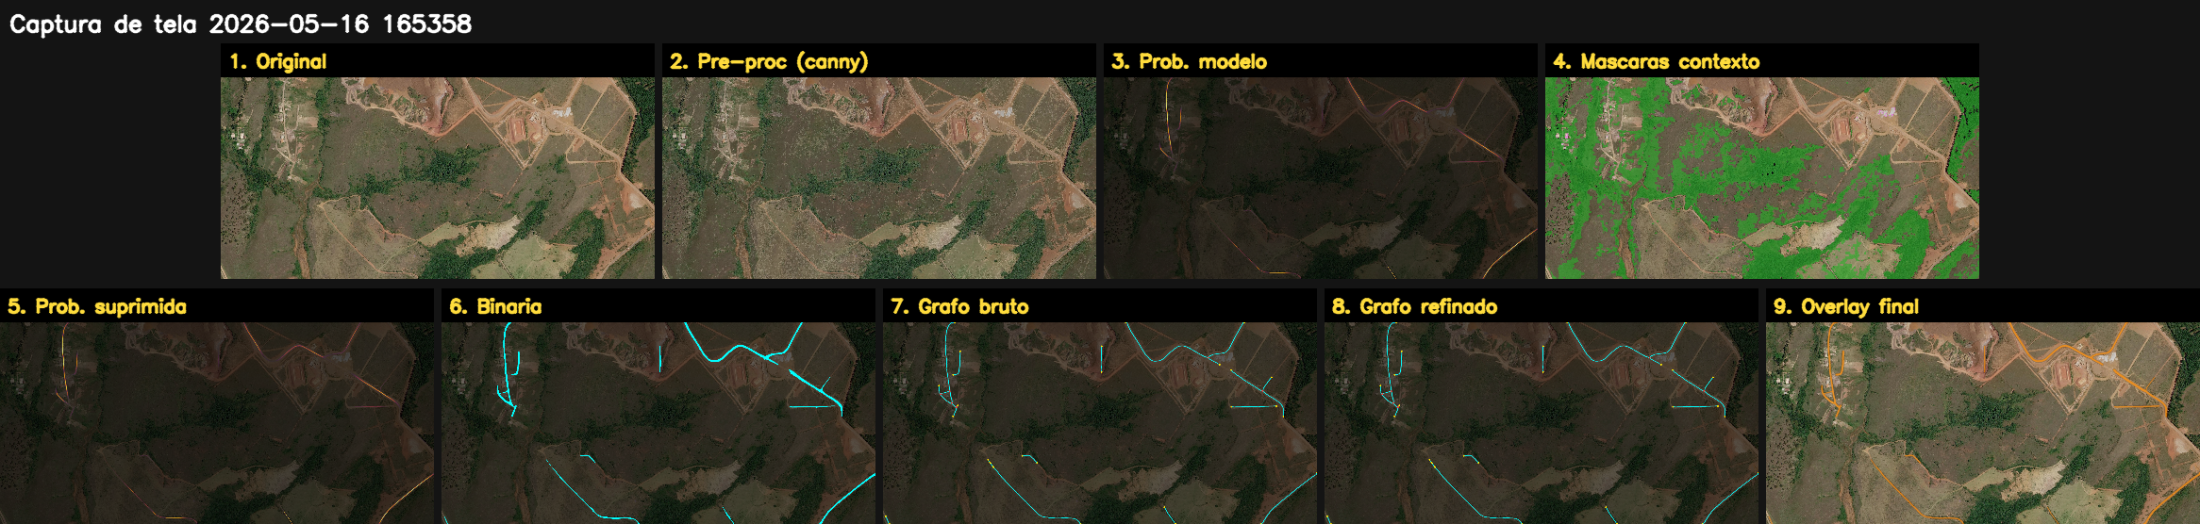
\includegraphics[width=\linewidth]{grid_2026-05-16_165358.png}
    \end{center}
    \footnotesize Cena rural mista. \textbf{Melhorou demais} após a detecção de domínio; vias de terra em laranja. \textbf{Faltam algumas ruas} de textura muito fraca --- limitação de \textit{recall} sem \textit{fine-tuning}.
\end{frame}

\begin{frame}{Limitações e melhorias futuras}
    \footnotesize
    \begin{itemize}\setlength{\itemsep}{3pt}
        \item \textbf{Sem \textit{fine-tuning}:} usamos pesos CityScale (urbano EUA). Em satélite rural escuro o sinal é fraco $\Rightarrow$ algumas vias de terra de baixa textura ficam incompletas (visto em 165358/131959).
        \item \textbf{Asfalto $\times$ terra} é \textbf{heurística} (cor + textura), não aprendida. Melhoria: cabeça supervisionada usando o atributo \texttt{paved} do SpaceNet.
        \item \textbf{Becos residenciais:} em áreas muito densas, alguns becos reais e vãos de telhado são indistinguíveis $\Rightarrow$ ainda há falsos positivos residuais.
        \item \textbf{Túneis:} via que entra em túnel é interrompida (trabalho futuro: portais virtuais).
    \end{itemize}
    \vspace{0.1cm}
    \begin{block}{Metodologia}
        \scriptsize Cada decisão é medida por um \textit{harness} de avaliação antes de ser adotada --- prioriza-se rigor experimental e generalização sobre ``funcionou nesta imagem''.
    \end{block}
\end{frame}

% =====================================================================
\section{Referências}
% =====================================================================
\begin{frame}{Referências}
    \footnotesize
    \begin{thebibliography}{9}
        \setbeamertemplate{bibliography item}[text]
        \bibitem{samroad} C. Hetang \textit{et al.}, ``Segment Anything Model for Road Network Graph Extraction,'' \textit{CVPRW}, 2024.
        \bibitem{samroadpp} Z. Yin \textit{et al.}, ``Towards Satellite Image Road Graph Extraction: A Global-Scale Dataset and A Novel Method,'' \textit{CVPR}, 2025.
        \bibitem{sam} A. Kirillov \textit{et al.}, ``Segment Anything,'' \textit{ICCV}, 2023.
        \bibitem{cldice} S. Shit \textit{et al.}, ``clDice -- a Novel Topology-Preserving Loss Function for Tubular Structure Segmentation,'' \textit{CVPR}, 2021.
        \bibitem{spacenet} SpaceNet Roads Challenge, \textit{spacenet.ai}, 2018.
    \end{thebibliography}
\end{frame}

\end{document}
